% !TeX root = ./11-handout.tex

\setcounter{section}{10}

\section{Multiple quantifiers \& \\ \qquad The Identity Predicate}

\begin{frame}
%\large

\scriptsize{\tableofcontents}

\end{frame}

\subsection{Two quantifiers}

\begin{frame}
  \frametitle{Formulas expressing relations}

\begin{itemize}[<+->]
  \item A formula $\metav{A}\qv{x}$ with one free variable expresses a \emph{property}
  \item A formula $\metav{B}\qr{x}{y}$ with two free variables expresses a \emph{relation}
  \item $\qt{\forall}{x}\qt{\forall}{y}\, \metav{B}\qr{x}{y}$ is a sentence: 
  \item It's true iff 
  \emph{every pair} of objects $\alpha$, $\beta$ stand in the relation expressed by $\metav{B}\qr{x}{y}$.
  \item $\qt{\exists}{x}\qt{\exists}{y}\, \metav{B}\qr{x}{y}$ is a sentence:
  \item It's true iff
  \emph{at least one pair} of objects $\alpha$, $\beta$ stand in the relation expressed by $\metav{B}\qr{x}{y}$.
\end{itemize}
\end{frame}

\begin{frame}
  \frametitle{Multiple uses of a single quantifier: $\forall$}

\begin{itemize}[<+->]
  \item $A\qr{x}{y}$: $x$ admires $y$.
  \item $\qt{\forall}{x}\qt{\forall}{y}\, A\qr{x}{y}$: for every pair $\langle
  \alpha,\beta\rangle$, $\alpha$ admires $\beta$.
  \item In other words: everyone admires everyone.
  \item Note: ``every pair'' includes pairs $\langle\alpha, \alpha\rangle$, i.e.,
  \item $\qt{\forall}{x}\qt{\forall}{y}\, A\qr{x}{y}$ is true only if all pairs $\langle \alert{\alpha, \alpha}\rangle$ satisfy $A\qr{x}{y}$.
  \item That means, everyone admires themselves, in addition to everyone else.
  \item So: $\qt{\forall}{x}\qt{\forall}{y}\, A\qr{x}{y}$ does \emph{not} symbolize ``everyone admires everyone \emph{else}.'' (To handle that, we'll need identity!)
\end{itemize}

\end{frame}

\begin{frame}
  \frametitle{Multiple uses of single quantifier: $\exists$}

\begin{itemize}[<+->]
  \item $\qt{\exists}{x}\qt{\exists}{y}\, A\qr{x}{y}$: for at least one pair $\langle \alpha,\beta\rangle$, $\alpha$ admires $\beta$.
  \item In other words: at least one person admires at least one person.
  \item Note: includes pairs $\langle\alpha, \alpha\rangle$, i.e.,
  \item $\qt{\exists}{x}\qt{\exists}{y}\, A\qr{x}{y}$ is already true if a single pair $\langle \alpha, \alpha\rangle$ satisfies $ A\qr{x}{y}$.
  \item That means, we could just have one person admiring themselves.
  \item So: $\qt{\exists}{x}\qt{\exists}{y}\, A\qr{x}{y}$ does \emph{not} symbolize ``someone admires someone \emph{else}.'' (again, for that, we'll need the identity predicate)
\end{itemize}
\end{frame}

\begin{frame}
    \frametitle{Alternating quantifiers}

\begin{enumerate}[<+->]
  \item $\qt{\forall}{x} \qt{\exists}{y} \, A\qr{x}{y}$
  \item<2->[] Everyone admires someone\\
    (possibly themselves)
  \item $\qt{\forall}{y} \qt{\exists}{x} \, A\qr{x}{y}$
  \item<3->[] Everyone is admired by someone\\
  (not necessarily the same person)
  \item $\qt{\exists}{x} \qt{\forall}{y} \, A\qr{x}{y}$
  \item<4->[] Someone admires everyone\\
  (including themselves)
  \item $\qt{\exists}{y} \qt{\forall}{x} \, A\qr{x}{y}$
  \item<5->[] Someone is admired by everyone\\
    (including themselves)
\end{enumerate}

\end{frame}

\begin{frame}
    \frametitle{Convergence vs. uniform convergence}

\begin{itemize}[<+->]
\item A function $f$ is \emph{point-wise continuous} if
\[
\qt{\forall}{\epsilon}\qt{\forall}{x}\qt{\forall}{y}\qt{\exists}{\delta}(\left|x - y\right| < \delta \to \left|f\qvp{x} - f\qvp{y}\right| < \epsilon)
\]
\item A function $f$ is \emph{uniformly continuous} if
\[
\qt{\forall}{\epsilon} \qt{\exists}{\delta} \qt{\forall}{x}\qt{\forall}{y}(\left|x - y\right| < \delta \to \left|f\qvp{x} - f\qvp{y}\right| < \epsilon)
\]
\end{itemize}

\end{frame}

\subsection{Multiple Determiners}

\begin{frame}
\frametitle{``Determiner phrases'' say what?}
%\large

\begin{itemize}[<+->]

\item Determiners: quantifiers and indefinite or definite articles \\ (also possessives and demonstratives)

\item e.g. many, some, a, the, his, their, this, that

\item Determiner phrases: combine a determiner with a (possibily modified) noun:

\item `all heroes'; `a cape'

\item `some woman'; `the donkey'

\end{itemize}
\end{frame}

\begin{frame}
  \frametitle{Symbolizing multiple determiners}

\begin{itemize}[<+->]
\item What if your sentence contains more than one determiner phrase?
\item Deal with each determiner separately!
\item Think of determiner phrase as replaced with name or variable---result has one less determiner.
\item When you're down to one determiner, apply known methods for single quantifiers.
\item This results in formulas that express properties or relations, but themselves contain quantifiers.
\end{itemize}
\end{frame}

\begin{frame}
    \frametitle{Two separate determiner phrases}

\begin{itemize}[<+->]
\item \textcolor{highlightB}{All heroes} wear \textcolor{highlightA}{a cape}
\item \textcolor{highlightB}{All heroes} satisfy ``$x$ wears \textcolor{highlightA}{a cape}'' \[
\textcolor{highlightB}{\qt{\forall}{x}(H\qv{x} \eif {}} \text{``$x$ wears \textcolor{highlightA}{a cape}''})
\]
\item $x$ wears \textcolor{highlightA}{a cape}\[
 \textcolor{highlightA}{\qt{\exists}{y}(E\qv{y} \land{}} R\qr{x}{y})
\]
\item Together:
\[
\textcolor{highlightB}{\qt{\forall}{x}(H\qv{x} \eif {}} \textcolor{highlightA}{\qt{\exists}{y}(E\qv{y} \land{}} R\qr{x}{y}))
\]
\end{itemize}
\end{frame}

\begin{frame}
    \frametitle{Determiner within determiner phrase}

\begin{itemize}[<+->]
\item \textcolor{highlightB}{All heroes who wear \textcolor{highlightA}{ a cape}} admire Greta.
\item All things that satisfy ``$x$ is a hero who wears \textcolor{highlightA}{a cape}'' admire Greta.
\[
\qt{\forall}{x} (\text{``x is a hero who wears a cape''} \eif A\qr{x}{g})
\]
\item $x$ is a hero who wears \textcolor{highlightA}{a cape}
\[
 H\qv{x} \land \qt{\exists}{y}(E\qv{y} \land R\qr{x}{y})
\]
\item Together:
\[
\qt{\forall}{x}((H\qv{x} \land \qt{\exists}{y}(E\qv{y} \land R\qr{x}{y})) \eif A\qr{x}{g})
\]
\end{itemize}
\end{frame}

\begin{frame}
    \frametitle{``Any'' is sometimes existential}

\begin{itemize}[<+->]
\item Any (every) cape is worn by a hero:
\[
\uncover<2->{\qt{\forall}{x}(E\qv{x} \eif \qt{\exists}{y}(H\qv{y} \land R\qr{y}{x}))}
\]\pause
\item No hero wears any cape:
\begin{align*}
\uncover<3->{\qt{\forall}{x}(H\qv{x} & \eif \enot\qt{\exists}{y}(E\qv{y} \land R\qr{x}{y}))} {}\\
\uncover<4->{\enot \qt{\exists}{x}(H\qv{x} & \eand \qt{\exists}{y}(E\qv{y} \land R\qr{x}{y}))}
\end{align*}
\item No hero wears every cape:
\begin{align*}
\uncover<5->{\qt{\forall}{x}(H\qv{x} & \eif \enot\qt{\forall}{y}(E\qv{y} \eif R\qr{x}{y}))}{}\\
\uncover<6->{\enot\qt{\exists}{x}(H\qv{x} & \eand \qt{\forall}{y}(E\qv{y} \eif R\qr{x}{y}))}
\end{align*}
\end{itemize}
\end{frame}

\subsection{The identity predicate}

\begin{frame}
  \frametitle{Greta admires everyone (else)}

\usetikzlibrary{arrows}
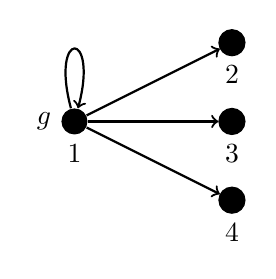
\begin{tikzpicture}
    \node[circle,fill,label={below:$1$},label={left:$g$}] (A) at (-1,0) {};
    \node[circle,fill,draw,label={below:$2$}] (B) at (1,1) {};
    \node[circle,fill,draw,label={below:$3$}] (C) at (1,0) {};
    \node[circle,fill,draw,label={below:$4$}] (D) at (1,-1) {};
    \draw[->,thick] (A) to[loop above,looseness=30] (A);
    \draw[->,thick] (A) -- (B);
    \draw[->,thick] (A) -- (C);
    \draw[->,thick] (A) -- (D);
\end{tikzpicture}
\hfill
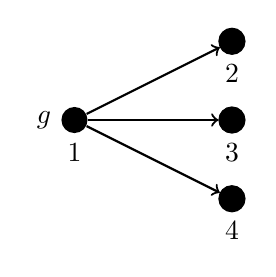
\begin{tikzpicture}
  \node[circle,fill,label={below:$1$},label={left:$g$}] (A) at (-1,0) {};
  \node[circle,fill,draw,label={below:$2$}] (B) at (1,1) {};
  \node[circle,fill,draw,label={below:$3$}] (C) at (1,0) {};
  \node[circle,fill,draw,label={below:$4$}] (D) at (1,-1) {};
  %\draw[->,thick] (A) to[loop above,looseness=30] (A);
  \draw[->,thick] (A) -- (B);
  \draw[->,thick] (A) -- (C);
  \draw[->,thick] (A) -- (D);
\end{tikzpicture}

Greta admires \hfill Greta admires\\
everyone. \hfill everyone \emph{else}.\\

\uncover<2->{\alert{$\qt{\forall}{x}\, A\qr{g}{x}$}}\hfill\uncover<3->{\alert{$\qt{\forall}{x}(\text{``$x$ is not Greta''} \eif A\qr{g}{x})$}}\\
\hfill\uncover<4->{\alert{$\qt{\forall}{x}(\enot x= g \eif A\qr{g}{x})$}}

\end{frame}

\begin{frame}
  \frametitle{The identity predicate}

  \begin{itemize}[<+->]
    \item A new, special two-place predicate: \emph{$=$}
    \begin{itemize}[<+->]
      \item Written between arguments, \emph{without parentheses}.
      \item Needs no mention in symbolization key.
      \item Always interpreted the same: extension of `$=$' is all pairs $\langle\alpha, \alpha\rangle$.
    \end{itemize}
    \bigskip
    \item `$a=b$' true iff `$a$' and `$b$' name one and the same object.
    \item $x=y$ satisfied by all and only the pairs $\langle \alpha,\alpha\rangle$.
    \item $\lnot x=y$ is satisfied by a pair $\langle
    \alpha,\beta\rangle$ iff $\alpha$ and $\beta$ are different objects.
  \end{itemize}
\end{frame}

\begin{frame}
 \frametitle{MISTAKES! Ungrammatical expressions with identity}
  \begin{itemize}[<+->]
   \item \textcolor{red}{$x = \lnot y$} is \textcolor{red}{not grammatical.} 
   \item[] $\lnot$ can only go in front of a formula, and $y$ is not one.
    \item\textcolor{red}{$\lnot(x=y)$} is also not grammatical.
    \item[] `$(x=y)$' is also not a formula.
    \item \textit{Carnap} will not tolerate this nonsense! Take heed! 
   \end{itemize}
\end{frame}


\begin{frame}
    \frametitle{`Something else' and `everything else'}

\begin{itemize}[<+->]
\item Remember: different variables do NOT entail different objects.
\item $\qt{\exists}{x}\qt{\exists}{y}\,A\qr{x}{y}$ doesn't mean that someone admires
someone else.
\item It just means that someone admires someone (possibly
themselves).
\item To symbolize ``someone else'' add $\lnot x\!\!=\!\!y$:
\[\color{highlightA}
\qt{\exists}{x}\qt{\exists}{y}(\lnot x\!\!=\!\!y \land A\qr{x}{y})\]
\item $\qt{\forall}{x}\qt{\forall}{y}\,A\qr{x}{y}$ says that everyone admires everyone
(including themselves).
\item To symbolize ``everyone admires everyone else'' add $\lnot x\!\!=\!\!y$:
\[\color{highlightA}
\qt{\forall}{x}\qt{\forall}{y}(\lnot x\!\!=\!\!y \eif A\qr{x}{y})\]
\end{itemize}
\end{frame}

\begin{frame}
  \frametitle{`Something else' and `everything else'}

\begin{itemize}[<+->]
\item The closest quantifier (typically) determines whether \\ \qquad you should use $\land$ or $\eif$: \\
\makebox[\textwidth]{$\qt{\forall}{x}\qt{\exists}{y}(\lnot x\!\!=\!\!y \eand A\qr{x}{y})$ \quad vs. \quad $\qt{\exists}{x}\qt{\forall}{y}(\lnot x\!\!=\!\!y \eif A\qr{x}{y})$} {}\\ 
\footnotesize{\qquad Everyone admires someone else vs. Someone admires everyone else}
%\[
%  \qt{\forall}{x}\qt{\exists}{y}(\lnot x\!\!=\!\!y \eand A\qr{x}{y}) \quad vs. \quad
%  \qt{\exists}{x}\qt{\forall}{y}(\lnot x\!\!=\!\!y \eif A\qr{x}{y})
%\]
%\item[] \makebox[\textwidth]{\footnotesize{Everyone admires someone else vs. Someone admires everyone else}}
\bigskip
\item If you have mixed domains, it works the same way:
\item Recall predicate `$P\qv{x}$': ``$x$ is a person''
\item Everyone admires someone \emph{else}:
\[\color{highlightA}
\qt{\forall}{x}(P\qv{x} \eif \qt{\exists}{y}((P\qv{y} \eand \enot x\!\!=\!\!y) \eand A\qr{x}{y}))
\]
\item Someone admires everyone \emph{else}:
\[\color{highlightA}
\qt{\exists}{x}(P\qv{x} \eand \qt{\forall}{y}((P\qv{y} \eand \enot x\!\!=\!\!y) \eif A\qr{x}{y})
\]
\end{itemize}
\end{frame}

\begin{frame}
  \frametitle{Other than, except}
  
  
  \begin{itemize}[<+->]
    \item ``\emph{Someone other than Greta} is a hero'':
    \item[] \emph{$\qt{\exists}{x}(\lnot x = g \eand H\qv{x})$}
    \item ``\emph{Everyone other than Greta} is a hero''; same as:
    \item ``\emph{Everyone except Greta} is a hero'':
    \item[] \emph{$\qt{\forall}{x}(\lnot x = g \eif H\qv{x})$}
    \end{itemize}
\end{frame}


\begin{frame}
  \frametitle{`No-one other than' vs. Singular ``only''}

  \begin{itemize}[<+->]
    \item ``\emph{No-one other than Greta} is a hero'':
    \item[] \emph{$\enot\qt{\exists}{x}(H\qv{x} \eand \enot x\!\!=\!\!g)$}
    \item[] \emph{$\qt{\forall}{x}(H\qv{x} \eif x\!\!=\!\!g)$}
    \item ``\emph{Only Greta} is a hero'':
    \item Content: No-one other than Greta is a hero, \emph{AND} Greta is a hero:
    \item[] \emph{$\qt{\forall}{x}(H\qv{x} \eif x\!\!=\!\!g) \eand H\qv{g}$}
    \item[] \emph{$\qt{\forall}{x}(H\qv{x} \eiff x\!\!=\!\!g)$}
    %JH: are these two symbolizations quantificationally equivalent? i.e. can i derive one from the other? think about---could be good exercise. alternativelY: is there a countermodel to equivalence
    %maybe they disagree in case nothing is a hero, latter is trivially true? whereas former requires g to be in extension of H. 
  \end{itemize}
  \end{frame}
  
\begin{frame}
    \frametitle{Uniqueness}

\begin{itemize}[<+->]
\item Non-unique: ``There is at least one hero'':
\[\color{highlightA}
\qt{\exists}{x}\, H\qv{x}
\]
\item Unique: ``There is exactly one hero'':
\begin{itemize}[<+->]
\item There's at least one hero, AND
\item There are no others:
\begin{align*}
\uncover<5->{\qt{\exists}{x}\, (H\qv{x} \land {}} & 
  \uncover<6->{\textcolor{highlightA}{\lnot \qt{\exists}{y}\, (\lnot y = x \land H\qv{y})})}\\
\uncover<7->{\qt{\exists}{x}\,(H\qv{x} \land {}} & 
\uncover<7->{\textcolor{highlightA}{\qt{\forall}{y}(H\qv{y} \to x\!\!=\!\!y)})}
\end{align*}
\item<8>Or more succinctly: 
$\color{highlightA}\qt{\exists}{x}\qt{\forall}{y}(H\qv{y} \eiff x\!\!=\!\!y)$
\end{itemize}
\end{itemize}
\end{frame}


\subsection{Numerical quantification}

\begin{frame}
    \frametitle{Numerical Quantification: $n$-many as `at least $n$'}

\begin{itemize}[<+->]
\item Cardinal numbers can be determiners:
\begin{itemize}
\item \emph{Three heroes} wear capes.
\end{itemize}
\item Not always clear if ``three heroes'' means \textcolor{highlightB}{exactly} vs. \emph{at least} three hero
\item We'll assume the \textcolor{highlightA}{latter}.%---the ``exactly'' is implicated, not implied. Why?
\begin{itemize}[<+->]
\item Do you have two dollars? Yes, I have two dollars. \\ (Uncontroversially true even if you have more than \$2)
%\item How much money do you have? I have two dollars. \\ (True but misleading if you have more.)
\end{itemize}
\item Using QL, we can express the following kinds of sentences:
\begin{itemize}[<+->]
\item \emph{At least $n$} people are \dots
\item \emph{Exactly $n$} people are \dots
\item \emph{At most $n$} people are \dots
\end{itemize}
\item i.e. we can count on QL! 
\end{itemize}
\end{frame}

\begin{frame}
    \frametitle{At least $n$}

\begin{itemize}[<+->]
\item At least 1 hero is inspiring:
\[
\alert{\qt{\exists}{x}(H\qv{x} \land I\qv{x})}
\]
\item At least 2 heroes are inspiring:
\[
\alert{\qt{\exists}{x}\qt{\exists}{y}}(\alert{\enot x\!\!=\!\!y \land ((H\qv{x} \land I\qv{x}) \land (H\qv{y} \land I\qv{y}))})
\]
\item At least 3 heroes are inspiring:
\begin{align*}
& \alert{\qt{\exists}{x}\qt{\exists}{y}\qt{\exists}{z}}\Big(\alert{(\enot x\!\!=\!\!y \land (\enot y = z \land \enot x = z)) \eand {}} \\
& \qquad \alert{\big((H\qv{x} \land I\qv{x}) \land ((H\qv{y} \land I\qv{y}) \eand (H\qv{z} \land I\qv{z}))\big)}\Big)
\end{align*}
\end{itemize}
\end{frame}


\begin{frame}
  \frametitle{At least $n$}

\begin{itemize}
\item There are at least $n$ $A$s, i.e. ``$\qt{\exists^{\ge n}}{x}\,A\qv{x}$'':
\begin{align*}
\qt{\exists}{x_1}\dots\qt{\exists}{x_n}\Big(\uncover<2->{(\enot x_1 = x_2 \land (\enot x_1 = x_3 \land \dots \land (\enot x_1 = x_n} & \uncover<2->{{} \land {}}\\
\uncover<2->{(\enot x_2 = x_3 \land \dots \land (\enot x_2 = x_n} & \uncover<2->{{} \land {}}\\
\uncover<2->{\ddots}\qquad &\\
\uncover<2->{\enot x_{n-1} = x_n)\dots)} & \uncover<2->{{} \land {}}\\
\uncover<3->{(A\qv{x_1} \land (A\qv{x_2} \land \dots \land A\qv{x_n})\dots)\Big)}
\end{align*}
\end{itemize}
\end{frame}

\begin{frame}
  \frametitle{At least $n$}

\begin{itemize}[<+->]
\item Note: must state that \emph{every pair} of variables is different, e.g.,
\begin{align*}
\qt{\exists}{x_1}\qt{\exists}{x_2}\qt{\exists}{x_3}(&(\enot x_1 = x_2 \land \enot x_2 = x_3) \land {}\\
& (H\qv{x_1} \land (H\qv{x_2} \land H\qv{x_3})))
\end{align*}
only says ``There are at least two heroes''!
\begin{itemize}[<+->]
  \item Take extension of $H\qv{x}$ to be: $1,2$
  \item Then $1$ can play role of $x_1$ and $x_3$, $2$ role of $x_2$.
  \item Both ``$\enot 1=2$'' and ``$\enot 2=3$'' are true.
\end{itemize}
\item At least $n$ $B$s are $C$s: substitute `$B\qv{x} \eand C\qv{x}$' for `$A\qv{x}$':
\[
\qt{\exists^{\ge n}}{x} (B\qv{x} \land C\qv{x})
\]
\end{itemize}
\end{frame}

\begin{frame}
    \frametitle{Exactly one (i.e. Uniqueness; see above)}

\begin{itemize}[<+->]
\item There is exactly one hero:
\[
\qt{\exists}{x}(H\qv{x} \land \lnot \qt{\exists}{y}(H\qv{y} \land \enot x\!\!=\!\!y))
\]
\item This is equivalent to:
\[
\qt{\exists}{x}(H\qv{x} \land \qt{\forall}{y}(H\qv{y} \to x\!\!=\!\!y))
\]
\item In general: ``$g$ has property $A$ \emph{uniquely}'':
\begin{align*}
A\qv{g} \land {} & \qt{\forall}{y}(A\qv{y} \to g\!\!=\!\!y)\\
\text{or just:\qquad} & \qt{\forall}{y}(A\qv{y} \eiff g\!\!=\!\!y)
\end{align*}
\end{itemize}
\end{frame}

\begin{frame}
  \frametitle{Exactly $n$}

\begin{itemize}
\item<1-> There are exactly $n$ $A$s, i.e. ``$\qt{\exists^{=n}}{x}\,A\qv{x}$'':
\begin{align*}
\qt{\exists}{x_1}\dots\qt{\exists}{x_n}\Big(\uncover<2->{(\enot x_1 = x_2 \land (\enot x_1 = x_3 \land \dots \land (\enot x_1 = x_n} & \uncover<2->{{} \land {}}\\
\uncover<2->{(\enot x_2 = x_3 \land \dots \land (\enot x_2 = x_n} & \uncover<2->{{} \land {}}\\
\uncover<2->{\ddots}\qquad &\\
\uncover<2->{\enot x_{n-1} = x_n)\dots)} & \uncover<3->{{} \land {}}\\
\uncover<presentation:3-4|handout:1>{(A\qv{x_1} \land (A\qv{x_2} \land \dots \land A\qv{x_n})\dots))} & \uncover<presentation:4|handout:1>{{} \eand {}}\\
\uncover<4->{\qt{\forall}{y}(A\qv{y} \only<presentation: 4|handout:1>{\emph{\eif}} \only<presentation: 5-|handout:2>{\textcolor{OGlyallpink}{\eiff}} (y = x_1 \lor \dots \lor y=x_n))\Big)}
\end{align*}
\item<6-> Exactly $n$ $B$s are $C$s:
\[
\qt{\exists^{=n}}{x} (B\qv{x} \land C\qv{x})
\]
\end{itemize}
\end{frame}

\begin{frame}
    \frametitle{At most $n$}

\begin{itemize}
\item<1-> There are \emph{at most $n$} $A$s $\Leftrightarrow$ There are
\emph{not at least $n+1$} $A$s
\[
\qt{\exists^{\alert{\le n}}}{x}\, A\qv{x} \Leftrightarrow \alert{\lnot} \qt{\exists^{\alert{\ge(n+1)}}}{x} \, A\qv{x}
\]
\item<2-> For instance: There are at most two heroes:
\begin{align*}
\uncover<2->{\lnot \qt{\exists}{x}\qt{\exists}{y}\qt{\exists}{z}((H\qv{x} \land (H\qv{y} \land H\qv{z}))}
& \uncover<2->{\land (\lnot x =y \land (\lnot x = z \land \lnot y = z)) )}\\
\uncover<3->{\qt{\forall}{x}\qt{\forall}{y}\qt{\forall}{z}((H\qv{x} \land (H\qv{y} \land H\qv{z}))
} &\uncover<3->{\eif (x =y \lor ( x = z \lor y = z)) )}
\end{align*}
\item<4-> $\lnot \qt{\exists^{\ge(n+1)}}{x} \, A\qv{x}$ is equivalent to:
\begin{align*}
\qt{\forall}{x_1}\dots\qt{\forall}{x_{n+1}} \textcolor{highlightA}{(}(A\qv{x_1} \land \dots \land A\qv{x_{n+1}}) \eif \qquad \\
\textcolor{OGlyallpink}{(}x_1 = x_2 \lor (x_1 = x_3 \lor \dots \lor (x_1 = x_{n+1} & {} \lor {}\\
(x_2 = x_3 \lor \dots \lor (x_2 = x_{n+1} & {} \lor {}\\
\ddots\qquad &\\
x_n = x_{n+1})\dots) & \textcolor{OGlyallpink}{)}\textcolor{highlightA}{)}
\end{align*}
\end{itemize}
\end{frame}

\subsection{Both `both' and `neither'}

\begin{frame}
    \frametitle{Schematizing `Both'}

\begin{itemize}
\item<1-> ``Both heroes inspire'': this means that 
\item[]<1-> There are \emph{exactly 2} heroes, and both inspire:
\begin{align*}
\qt{\exists}{x}\qt{\exists}{y}\Big(\uncover<2->{((\enot x\!\!=\!\!y \land (H\qv{x} \land H\qv{y}))} & 
\uncover<3->{{} \land {}}\\
\uncover<3->{\qt{\forall}{z}(H\qv{z} \to (z = x \lor z = y)))} & \uncover<4->{{}\land {}}\\
\uncover<4->{(I\qv{x} \eand I\qv{y})\Big)}&
\end{align*}
\item<5-> Note: ``Both heroes inspire'' implies ``There are exactly two inspiring heroes'', but not vice versa!
\item<6-> e.g. if there are exactly two inspiring heros and one (or more) not-inspiring hero(s)
%b/c `exactly two inspiring heros' could be true while there are more than two heros, e.g. three heros and on is uninspiring
\end{itemize}
\end{frame}

\begin{frame}
    \frametitle{Schematizing `Neither'}

\begin{itemize}[<+->]
\item ``Neither hero inspires'': this means that 
\item[] There are \emph{exactly 2} heroes, and neither of them inspires:
\begin{align*}
\qt{\exists}{x}\qt{\exists}{y}\Big(\textcolor{OGlyallpink}{(}(\lnot x\!\!=\!\!y \land (H\qv{x} \land H\qv{y})) & {}\land {}\\
\qt{\forall}{z}(H\qv{z} \to (z = x \lor z = y))\textcolor{OGlyallpink}{)} &{} \land {}\\
(\enot I\qv{x} \eand \enot I\qv{y})\Big)&
\end{align*}
\end{itemize}
\end{frame}

\subsection{`The' Definite Description}

\begin{frame}
    \frametitle{Definite descriptions}

\begin{itemize}[<+->]
\item Definite description: \emph{the so-and-so}
\item Russell's analysis of definite description: to say\\[1ex]
\centerline{``The $A$ is B''}
is to say:
\item There is something, which:
\begin{itemize}[<+->]
\item is $A$,
\item is the \emph{only} $A$ (i.e. the unique thing that is $A$),
\item is $B$.
\end{itemize}
\item In QL:
\[
\qt{\exists}{x}(A\qv{x} \land \qt{\forall}{y}(A\qv{y} \to x\!\!=\!\!y) \land B\qv{x})
\]
\item or more succinctly:
\[
\qt{\exists}{x}\qt{\forall}{y}\big((A\qv{y} \eiff x\!\!=\!\!y) \land B\qv{x}\big)
\]
\end{itemize}
\end{frame}



\begin{frame}
\frametitle{Example: `The author of Waverley is blah'}
%\large

\begin{itemize}[<+->]

\item Schematize ``The author of \textit{Waverley} is Scottish'':

\item Use the following symbolization key:

\item $Ax$: x is an author; $Wxz$: x wrote z; $Sx$: x is Scottish; $\ell$: \textit{Waverley}
\item[]
\[
\qt{\exists}{x}(A\qv{x} \land Wx\ell \land \qt{\forall}{y}( (A\qv{y} \land Wy\ell) \to x\!\!=\!\!y) \land S\qv{x})
\]

%Perhaps why Russell used `the author of Waverley' (i.e. scottish poet/novelist Sir Walter Scott) as his running example: Scott published Waverley anonymously and then subsequent novels as being "by the author of Waverley".

\end{itemize}
\end{frame}

\begin{frame}
\frametitle{``The'' vs. ``exactly one''}

\begin{itemize}[<+->]
\item Compare:
\begin{enumerate}[<+->]
\item The hero inspires:
\[\qt{\exists}{x}(H\qv{x} \land \qt{\forall}{y}(H\qv{y} \to x\!\!=\!\!y) \land I\qv{x})\]
\item There is exactly one inspiring hero:
\[\qt{\exists}{x}(H\qv{x} \land I\qv{x} \land \qt{\forall}{y}((H\qv{y} \alert{{}\land I\qv{y}}) \to x\!\!=\!\!y) )\]
\end{enumerate}
\item (2) can be true without (1), but not vice versa.
\item (Namely when there is exactly one inspiring hero, but also a non-inspiring hero.)
\item So (1) entails (2), but not vice versa.
\end{itemize}
\end{frame}

\begin{frame}
    \frametitle{Strawson's analysis (presuppositional theories)}

\begin{itemize}[<+->]
\item According to Russell, ``The hero wears a cape'' is \emph{false} if there is no hero, or if there is more than one.
\item Consider: ``the present King of France is bald.''
\item P. F. Strawson disagrees with these truth conditions. \\ Rather, we only succeed in making a statement \textcolor{OGlyallpink}{if there is a unique hero} (or a unique king of France).
\item ``There is a unique hero'' is not part of what is \emph{said} by a definite description, but is only \textcolor{OGlyallpink}{presupposed}.
\end{itemize}
\end{frame}

\begin{frame}
  \frametitle{Singular possessive (a definite description)}

  \begin{itemize}[<+->]
    \item Singular possessives form noun phrases, e.g., ``Joe's cape''
    \item They work like definite descriptions: \\ Joe's cape is the cape Joe owns.
    E.g.:
    \begin{itemize}
      \item ``Autumn wears \alert{Joe's cape}'' symbolizes the same as:
      \item[] ``Autumn wears \alert{the cape that Joe owns}'':
      \item[]
      \begin{align*}
        \qt{\exists}{x}\Big(& \uncover<6->{\textcolor{OGlyallpink}{(}(E\qv{x} \land O\qr{j}{x}) \land {}}\\
        & \uncover<7->{\qt{\forall}{y}((E\qv{y} \land O\qr{j}{y}) \eif x\!\!=\!\!y)\textcolor{OGlyallpink}{)} \land {}}\\
        & \uncover<8->{W\qr{a}{x}\Big)}
      \end{align*}
    \end{itemize}
  \end{itemize}
\end{frame}

\begin{frame}
  \frametitle{Singular vs. plural possessive}

  \begin{itemize}[<+->]
    \item Compare \emph{plural} possessives: those are `$\forall$'s':
    \bigskip
    \begin{itemize}[<+->]
      \item ``Autumn wears \alert{Joe's cape\textbf{s}}'' symbolizes the same
      as:
      \item[] ``Autumn wears every cape that Joe owns'':
      \[\qt{\forall}{x}\big((E\qv{x} \land O\qr{j}{x}) \eif W\qr{a}{x}\big)\]
    \end{itemize}
    \item So plural possessives are NOT definite descriptions. 
  \end{itemize}
\end{frame}


\subsection{Using quantifiers to express properties}

\begin{frame}
\frametitle{Our symbolization key}

    \begin{ekey}
    \item[$Domain$] people alive in \year{} and items of clothing
    \item[a] Autumn
    \item[g] Greta
    \item[P\qv{x}] \gap{x} is a person
    \item[L\qv{x}] \gap{x} is an item of clothing.
    \item[E\qv{x}] \gap{x} is a cape
    \item[R\qr{x}{y}] \gap{x} wears \gap{y}
    \item[H\qv{x}] \gap{x} is a hero
    \item[I\qv{x}] \gap{x} inspires
    \item[Y\qr{x}{y}] \gap{x} is younger than \gap{y}
    \item[A\qr{x}{y}] \gap{x} admires \gap{y}
    \item[O\qr{x}{y}] \gap{x} owns \gap{y}
    \end{ekey}
\end{frame}


\begin{frame}
  \frametitle{Expressing properties, revisited}
    \begin{itemize}[<+->]
      \item One-place predicates express properties, e.g.,
      \item[] $H\qv{x}$ expresses property ``being a hero''
      \item Combinations of predicates (with connectives, names) can
      express derived properties, e.g.,
      \begin{itemize}[<+->]
        \item[] $A\qr{x}{g}$ expresses ``$x$ admires Greta''
        \item[] $H\qv{x} \eand C\qv{x}$ expresses ``$x$ is a hero who wears a cape''
      \end{itemize}
    \item Using quantifiers, we can express even more complex
    properties, e.g.,
    \item[] $\qt{\exists}{y}(P\qv{y} \eand A\qr{x}{y})$ expresses ``$x$ admires someone''
    \end{itemize}
  \end{frame}
  
  \begin{frame}
    \frametitle{Finding, using properties expressed}
  
  \begin{itemize}[<+->]
    \item If you can say it for Greta, you can say it for $x$.
    \begin{itemize}[<+->]
      \item Greta admires a hero.
      \item[] \alert{$\qt{\exists}{y}(H\qv{y} \eand A\qr{g}{y})$}
      \item $x$ admires a hero.
      \item[] \alert{$\qt{\exists}{y}(H\qv{y} \eand A\qr{x}{y})$}
    \end{itemize}
    \item If you can say it for $x$, you can say it for Greta.
    \begin{itemize}[<+->]
      \item $x$ wears a cape.
      \item[] \alert{$\qt{\exists}{y}(E\qv{y} \eand R\qr{x}{y})$}
      \item Greta wears a cape.
      \item[] \alert{$\qt{\exists}{y}(E\qv{y} \eand R\qr{g}{y})$}
    \end{itemize}
  \end{itemize}
  \begin{ekey}\scriptsize
    \item[E\qv{x}] \gap{x} is a cape
    \item[R\qr{x}{y}] \gap{x} wears \gap{y}
  \end{ekey}
  \end{frame}
  
  \begin{frame}
  \frametitle{Examples}
  
  \begin{itemize}[<+->]
    \item $x$ wears a cape.
    \item[] \alert{$\qt{\exists}{y}(E\qv{y} \eand R\qr{x}{y})$}
    \item $x$ is admired by everyone.
    \item[] \alert{$\qt{\forall}{y}(P\qv{y} \eif A\qr{y}{x})$}
    \item $x$ admires a hero.
    \item[] \alert{$\qt{\exists}{y}(H\qv{y} \eand A\qr{x}{y})$}
    \item $x$ admires only heroes.
    \item[] \alert{$\qt{\forall}{y}(A\qr{x}{y} \eif H\qv{y})$}
    \item $x$ is unclothed (i.e. naked).
    \item[] \alert{$\enot\qt{\exists}{y}(L\qv{y} \eand R\qr{x}{y})$}\\
     \alert{$\qt{\forall}{y}(L\qv{y} \eif \enot R\qr{x}{y})$}
  \end{itemize}
  
  {\scriptsize
  \begin{tabular}{llll}
    $P\qv{x}$ & \gap{x} is a person &
    $L\qv{x}$ & \gap{x} is an item of clothing\\
    $E\qv{x}$ & \gap{x} is a cape &
    $R\qr{x}{y}$ & \gap{x} wears \gap{y}
  \end{tabular}}
  \end{frame}

\subsection{Multiple determiners: worked example}



\begin{frame}
    \frametitle{Mary Astell, 1666--1731}

\begin{columns}
\begin{column}{3cm}
\pgfimage[height=4cm]{../assets/astell}
\end{column}
\begin{column}{7cm}
\begin{itemize}
\item British political philosopher
\item \textit{Some Reflections upon Marriage} (1700)
\item In preface to 3rd ed. 1706 reacts to William Nicholls' claim (in \textit{The Duty of Inferiors
towards their Superiors, in Five Practical Discourses} (London 1701), Discourse IV: The Duty of Wives to their
Husbands), that women are naturally inferior to men.
\end{itemize}
\end{column}
\end{columns}
\end{frame}



\begin{frame}
    \frametitle{Astell TL;DR}

\begin{itemize}[<+->]
  \item What can Nicholls possibly mean by ``women are naturally inferior to men''?
  \item It can't be that some woman is inferior to some man, since
  that's ``no great discovery.''
  \item After all, surely some men are inferior to some women.
  \item The obviously intended meaning must be: \emph{all} women are
  inferior to \emph{all} men.
  \item But that can't be right, for then ``the greatest Queen ought
  not to command but to obey her Footman.''
  \item It can't even be just: \emph{all} women are inferior to
  \emph{some} men.
  \item Since ``had they been pleased to remember their Oaths of
  Allegiance and Supremacy, they might have known that \textit{One}
  Woman is superior to \textit{All} the Men in these Nations.''
\end{itemize}

\end{frame}

\begin{frame}
    \frametitle{Symbolizing Astell}

\begin{itemize}[<+->]
\item \textcolor{highlightB}{ Some woman} is superior to \textcolor{highlightA}{ every man}
\item \textcolor{highlightB}{ Some woman} satisfies ``$x$ is superior to
\textcolor{highlightA}{ every man}''
\[\textcolor{highlightB}{\qt{\exists}{x}(W\qv{x} \land {}}\text{``$x$ is superior to \textcolor{highlightA}{every man}''})\]
\item $x$ is superior to \textcolor{highlightA}{ every man}
\[
\textcolor{highlightA}{\qt{\forall}{y}(M\qv{y} \eif {}}S\qr{x}{y})
\]
\item Together:
\[
\textcolor{highlightB}{\qt{\exists}{x}(W\qv{x} \land{}} \textcolor{highlightA}{\qt{\forall}{y}(M\qv{y} \to {}}S\qr{x}{y})\textcolor{highlightB}{)}
\]
\end{itemize}
\end{frame}

\begin{frame}
    \frametitle{Formalizing Astell}

\begin{itemize}[<+->]
\item Some woman is superior to some man.
\item[] \alert{$\qt{\exists}{x}(W\qv{x} \land \qt{\exists}{y}(M\qv{y} \land S\qr{x}{y}))$}
\item Every woman is superior to every man.
\item[] \alert{$\qt{\forall}{x}(W\qv{x} \to \qt{\forall}{y}(M\qv{y} \to S\qr{x}{y}))$}
\item Every woman is superior to some man.
\item[]\alert{$\qt{\forall}{x}(W\qv{x} \to \qt{\exists}{y}(M\qv{y} \land S\qr{x}{y}))$}
\item Some woman is superior to every man.
\item[] \alert{$\qt{\exists}{x}(W\qv{x} \land \qt{\forall}{y}(M\qv{y} \to S\qr{x}{y}))$}
\end{itemize}
\end{frame}





\subsection{Quantifier scope ambiguity}

\begin{frame}
  \frametitle{More scope ambiguity}

\begin{itemize}[<+->]
\item ``Autumn and Greta admire Isra or Luisa.''
\item Two logically distinct, natural readings:
\item[1)] Autumn admires Isra or Luisa, \emph{and} so does Greta.
\begin{align*}
(A\qr{a}{i} \lor {} & A\qr{a}{l}) \emph{\land} {}\\
(A\qr{g}{i} \lor {} & A\qr{g}{l})
\end{align*}
\item[2)] Autumn and Greta both admire Isra, \textcolor{highlightB}{or} they both admire Luisa.
\begin{align*}
(A\qr{a}{i} \land {} & A\qr{g}{i}) \textcolor{highlightB}{\lor} {}\\
(A\qr{a}{l} \land {} & A\qr{g}{l})
\end{align*}
\end{itemize}

\end{frame}


\begin{frame}
    \frametitle{Negation and the quantifiers}

\begin{itemize}[<+->]
\item ``All heroes don't inspire''
\begin{itemize}[<+->]
\item Denial of ``all heroes inspire''. Ask: ``Do all heroes inspire\\
(Answer: No, \textit{it's not the case that} all heroes inspire '')\pauses %No, all heroes don't inspire
\begin{align*}
\lnot\qt{\forall}{x}(H\qv{x} & {} \to I\qv{x}) \\
\qt{\exists}{x}(H\qv{x} & {} \land\lnot I\qv{x})
\end{align*}
\item All heroes are not inspiring, i.e.,\\
No heroes inspire\pauses
\begin{align*}
\qt{\forall}{x}(H\qv{x} & {} \to \lnot I\qv{x}) \\
\lnot\qt{\exists}{x}(H\qv{x} & {}\land I\qv{x})
\end{align*}
\end{itemize}
\end{itemize}
\end{frame}

\begin{frame}
    \frametitle{Multiple quantifiers and ambiguity}

\begin{itemize}[<+->]
\item ``All heroes wear a cape''
\begin{itemize}[<+->]
\item ``A cape'' in the scope of ``all heroes'', i.e.,\\
``For every hero, there is a cape they wear''\pauses
\[
\qt{\forall}{x}(H\qv{x} \to \qt{\exists}{y}(E\qv{y} \land R\qr{x}{y}))
\]
\[
\qt{\forall}{x}\qt{\exists}{y}(H\qv{x} \to (E\qv{y} \land R\qr{x}{y}))
\]
\item ``All heroes'' in scope of ``a cape'', i.e.,\\
``There is a cape which every hero wears''\pauses
\[
\qt{\exists}{y}(E\qv{y} \land \qt{\forall}{x}(H\qv{x} \to R\qr{x}{y}))
\]
\[
\qt{\exists}{y}\qt{\forall}{x}(E\qv{y} \land (H\qv{x} \to R\qr{x}{y}))
\]
\end{itemize}

\item A (probably bad) joke: ``Every day, a tourist is mugged on the streets of New York. He's going through a lot of wallets.'' %how does he keep getting the funds to buy a new wallet? kind people are donating their wallets to him. 

%\item Compare the joke: ``Every day, a tourist is mugged on the streets of New York. We will interview him tonight.'' %%JH: no idea how this is a joke??? is it a riff on `every day' vs. `tonight'?
%or is the riff on scope ambiguity: joke interpt is that there is a particular tourist who is mugged every day. so i tried to improve the joke to make it possibly funny? 
\end{itemize}
\end{frame}


\subsection{\quad Donkey sentences}

\begin{frame}
    \frametitle{Happy farmers}

``Every farmer who owns a donkey is happy''

\begin{itemize}[<+->]
\item Step-by-step symbolization: ``All $A$s are $B$s''
\item $x$ is a farmer who owns a donkey \dots\[
F\qv{x} \land \qt{\exists}{y}(D\qv{y} \land O\qr{x}{y})
\]
\item \textcolor{highlightA}{Every} farmer who owns a donkey \textcolor{highlightA}{is happy}
\[
\textcolor{highlightA}{\qt{\forall}{x}(}\textcolor{OGlyallpink}{(}F\qv{x} \land \qt{\exists}{y}(D\qv{y} \land O\qr{x}{y})\textcolor{OGlyallpink}{)} \textcolor{highlightA}{\eif H\qv{x})}
\]
\item Notice how `a donkey' is bound by an existential here
\end{itemize}
\end{frame}

\begin{frame}
    \frametitle{Unhappy donkeys :( }

``Every farmer who owns a donkey beats it''

\begin{itemize}[<+->]
\item Step-by-step symbolization: ``All As are Bs''
\item $x$ is a farmer who owns a donkey \dots\[
F\qv{x} \land \qt{\exists}{y}(D\qv{y} \land O\qr{x}{y})
\]
\item \textcolor{highlightA}{Every} farmer who owns a donkey \textcolor{highlightA}{beats} \textcolor{highlightB}{it}:
\[
\textcolor{highlightA}{\qt{\forall}{x}(}\textcolor{OGlyallpink}{(}F\qv{x} \land \qt{\exists}{y}(D\qv{y} \land O\qr{x}{y})\textcolor{OGlyallpink}{)} \textcolor{highlightA}{\to B\qr{x}{\textcolor{highlightB}{y}})}
\]
\item PROBLEM: `\textcolor{highlightB}{y}' is unbound! So this is not a QL sentence. Gasp! 
\end{itemize}
\end{frame}

\begin{frame}
\frametitle{Save the donkeys: a failed attempt}
%\large

\begin{itemize}[<+->]

\item This was our problem: a donkey lay beaten and \textcolor{highlightB}{unbound}:
\[
\textcolor{highlightA}{\qt{\forall}{x}(}\textcolor{OGlyallpink}{(}F\qv{x} \land \qt{\exists}{y}(D\qv{y} \land O\qr{x}{y})\textcolor{OGlyallpink}{)} \textcolor{highlightA}{\to B\qr{x}{\textcolor{highlightB}{y}})}
\]

\item Can we simply extend the scope of the existential? 
\[
\textcolor{highlightA}{\qt{\forall}{x}}\textcolor{highlightB}{\qt{\exists}{y}(}\textcolor{OGlyallpink}{(}F\qv{x} \land (D\qv{y} \land O\qr{x}{y})\textcolor{OGlyallpink}{)} \textcolor{highlightA}{\to B\qr{x}{\textcolor{highlightB}{y)}}}
\]

\item `y' is now bound, but alas, this sentence is trivially true:

\item Provided at least one thing in our UD is not a donkey, that thing makes the antecedent of the conditional false, making the conditional trivially true, for any $x$. 

\item[] In particular, our farmer is not a donkey.
\item[] But he still sounds like kind of a jack@\$\$! 





\end{itemize}
\end{frame}

\begin{frame}
    \frametitle{Symbolizing donkey sentences}

``Every farmer who owns a donkey beats it''\pauses

\begin{itemize}[<+->]
\item When is it false that every farmer who owns a donkey beats it? \pauses
If there's a farmer who owns a donkey but doesn't beat it. Deny that! \pauses
\[
\alert{\lnot\qt{\exists}{x}(F\qv{x} \land \qt{\exists}{y}(D\qv{y} \land O\qr{x}{y} \land \lnot B\qr{x}{y}))}
\]
\item For every farmer and every donkey they own: the farmer beats the donkey.
\[
\alert{\qt{\forall}{x}\qt{\forall}{y}((F\qv{x} \land (D\qv{y} \eand O\qr{x}{y})) \to B\qr{x}{y})}
\]
\item Every farmer beats every donkey they own.
\[
\alert{\qt{\forall}{x}(F\qv{x} \to \qt{\forall}{y}((D\qv{y} \land O\qr{x}{y}) \to B\qr{x}{y}))}
\]
%%JH: but still seems like we're limited: I can here the reading where the sentence means the farmer beats only one of his donkies!
\item But what about the case where at least one farmer with a donkey beats only one of his donkeys? $\#$Quitting
\end{itemize}
\end{frame}
